\chapter{Shortest paths}

\index{lyhin polku@lyhin polku}

Lyhimmän polun etsiminen alkusolmusta loppusolmuun
on keskeinen verkko-ongelma, joka esiintyy usein
käytännön tilanteissa.
Esimerkiksi tieverkostossa
luonteva ongelma on selvittää,
mikä on lyhin reitti kahden kaupungin välillä,
kun tiedossa ovat kaupunkien väliset tiet ja niiden pituudet.

Jos verkon kaarilla ei ole painoja,
polun pituus on sama kuin kaarten
määrä polulla, jolloin lyhimmän polun
voi etsiä leveyshaulla.
Tässä luvussa keskitymme kuitenkin
tapaukseen, jossa kaarilla on painot.
Tällöin lyhimpien polkujen etsimiseen
tarvitaan kehittyneempiä algoritmeja.

\section{Bellman–Fordin algoritmi}

\index{Bellman–Fordin algoritmi}

\key{Bellman–Fordin algoritmi} etsii
lyhimmän polun alkusolmusta
kaikkiin muihin verkon solmuihin.
Algoritmi toimii kaikenlaisissa verkoissa,
kunhan verkossa ei ole sykliä,
jonka kaarten yhteispaino on negatiivinen.
Jos verkossa on negatiivinen sykli,
algoritmi huomaa tilanteen.

Algoritmi pitää yllä etäisyysarvioita
alkusolmusta kaikkiin muihin verkon solmuihin.
Alussa alkusolmun etäisyysarvio on 0
ja muiden solmujen etäisyys\-arvio on ääretön.
Algoritmi parantaa arvioita
etsimällä verkosta kaaria,
jotka lyhentävät polkuja,
kunnes mitään arviota ei voi enää parantaa.

\subsubsection{Esimerkki}

Tarkastellaan Bellman–Fordin
algoritmin toimintaa seuraavassa verkossa:
\begin{center}
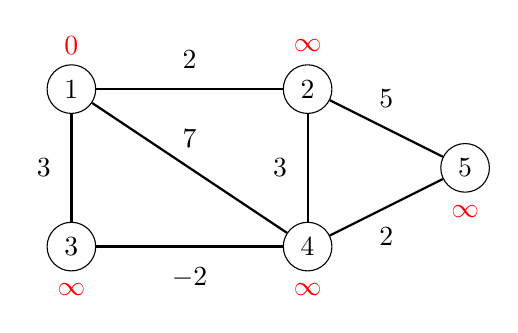
\begin{tikzpicture}
\node[draw, circle] (1) at (1,3) {1};
\node[draw, circle] (2) at (4,3) {2};
\node[draw, circle] (3) at (1,1) {3};
\node[draw, circle] (4) at (4,1) {4};
\node[draw, circle] (5) at (6,2) {5};
\node[color=red] at (1,3+0.55) {$0$};
\node[color=red] at (4,3+0.55) {$\infty$};
\node[color=red] at (1,1-0.55) {$\infty$};
\node[color=red] at (4,1-0.55) {$\infty$};
\node[color=red] at (6,2-0.55) {$\infty$};
\path[draw,thick,-] (1) -- node[font=\small,label=above:2] {} (2);
\path[draw,thick,-] (1) -- node[font=\small,label=left:3] {} (3);
\path[draw,thick,-] (3) -- node[font=\small,label=below:$-2$] {} (4);
\path[draw,thick,-] (2) -- node[font=\small,label=left:3] {} (4);
\path[draw,thick,-] (2) -- node[font=\small,label=above:5] {} (5);
\path[draw,thick,-] (4) -- node[font=\small,label=below:2] {} (5);
\path[draw,thick,-] (1) -- node[font=\small,label=above:7] {} (4);
\end{tikzpicture}
\end{center}
Verkon jokaiseen solmun viereen on merkitty etäisyysarvio.
Alussa alkusolmun etäisyysarvio on 0
ja muiden solmujen etäisyysarvio on
ääretön.

Algoritmi etsii verkosta kaaria,
jotka parantavat etäisyysarvioita.
Aluksi kaikki solmusta 0 lähtevät kaaret
parantavat arvioita:
\begin{center}
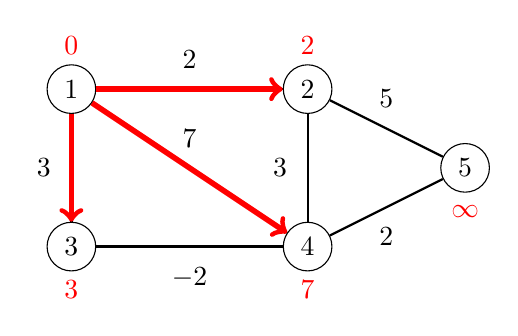
\begin{tikzpicture}
\node[draw, circle] (1) at (1,3) {1};
\node[draw, circle] (2) at (4,3) {2};
\node[draw, circle] (3) at (1,1) {3};
\node[draw, circle] (4) at (4,1) {4};
\node[draw, circle] (5) at (6,2) {5};
\node[color=red] at (1,3+0.55) {$0$};
\node[color=red] at (4,3+0.55) {$2$};
\node[color=red] at (1,1-0.55) {$3$};
\node[color=red] at (4,1-0.55) {$7$};
\node[color=red] at (6,2-0.55) {$\infty$};
\path[draw,thick,-] (1) -- node[font=\small,label=above:2] {} (2);
\path[draw,thick,-] (1) -- node[font=\small,label=left:3] {} (3);
\path[draw,thick,-] (3) -- node[font=\small,label=below:$-2$] {} (4);
\path[draw,thick,-] (2) -- node[font=\small,label=left:3] {} (4);
\path[draw,thick,-] (2) -- node[font=\small,label=above:5] {} (5);
\path[draw,thick,-] (4) -- node[font=\small,label=below:2] {} (5);
\path[draw,thick,-] (1) -- node[font=\small,label=above:7] {} (4);

\path[draw=red,thick,->,line width=2pt] (1) -- (2);
\path[draw=red,thick,->,line width=2pt] (1) -- (3);
\path[draw=red,thick,->,line width=2pt] (1) -- (4);
\end{tikzpicture}
\end{center}
Sitten kaaret $2 \rightarrow 5$ ja $3 \rightarrow 4$
parantavat arvioita:
\begin{center}
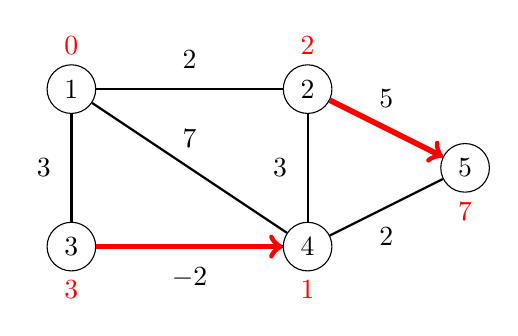
\begin{tikzpicture}
\node[draw, circle] (1) at (1,3) {1};
\node[draw, circle] (2) at (4,3) {2};
\node[draw, circle] (3) at (1,1) {3};
\node[draw, circle] (4) at (4,1) {4};
\node[draw, circle] (5) at (6,2) {5};
\node[color=red] at (1,3+0.55) {$0$};
\node[color=red] at (4,3+0.55) {$2$};
\node[color=red] at (1,1-0.55) {$3$};
\node[color=red] at (4,1-0.55) {$1$};
\node[color=red] at (6,2-0.55) {$7$};
\path[draw,thick,-] (1) -- node[font=\small,label=above:2] {} (2);
\path[draw,thick,-] (1) -- node[font=\small,label=left:3] {} (3);
\path[draw,thick,-] (3) -- node[font=\small,label=below:$-2$] {} (4);
\path[draw,thick,-] (2) -- node[font=\small,label=left:3] {} (4);
\path[draw,thick,-] (2) -- node[font=\small,label=above:5] {} (5);
\path[draw,thick,-] (4) -- node[font=\small,label=below:2] {} (5);
\path[draw,thick,-] (1) -- node[font=\small,label=above:7] {} (4);

\path[draw=red,thick,->,line width=2pt] (2) -- (5);
\path[draw=red,thick,->,line width=2pt] (3) -- (4);
\end{tikzpicture}
\end{center}
Lopuksi tulee vielä yksi parannus:
\begin{center}
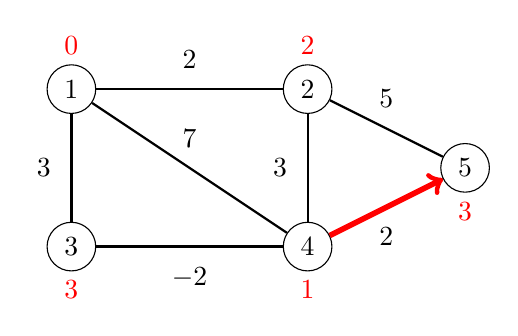
\begin{tikzpicture}
\node[draw, circle] (1) at (1,3) {1};
\node[draw, circle] (2) at (4,3) {2};
\node[draw, circle] (3) at (1,1) {3};
\node[draw, circle] (4) at (4,1) {4};
\node[draw, circle] (5) at (6,2) {5};
\node[color=red] at (1,3+0.55) {$0$};
\node[color=red] at (4,3+0.55) {$2$};
\node[color=red] at (1,1-0.55) {$3$};
\node[color=red] at (4,1-0.55) {$1$};
\node[color=red] at (6,2-0.55) {$3$};
\path[draw,thick,-] (1) -- node[font=\small,label=above:2] {} (2);
\path[draw,thick,-] (1) -- node[font=\small,label=left:3] {} (3);
\path[draw,thick,-] (3) -- node[font=\small,label=below:$-2$] {} (4);
\path[draw,thick,-] (2) -- node[font=\small,label=left:3] {} (4);
\path[draw,thick,-] (2) -- node[font=\small,label=above:5] {} (5);
\path[draw,thick,-] (4) -- node[font=\small,label=below:2] {} (5);
\path[draw,thick,-] (1) -- node[font=\small,label=above:7] {} (4);

\path[draw=red,thick,->,line width=2pt] (4) -- (5);
\end{tikzpicture}
\end{center}

Tämän jälkeen mikään kaari
ei paranna etäisyysarvioita.
Tämä tarkoittaa, että etäisyydet
ovat lopulliset, eli joka solmussa
on nyt pienin etäisyys alkusolmusta
kyseiseen solmuun.

Esimerkiksi pienin etäisyys 3
solmusta 1 solmuun 5 toteutuu käyttämällä
seuraavaa polkua:

\begin{center}
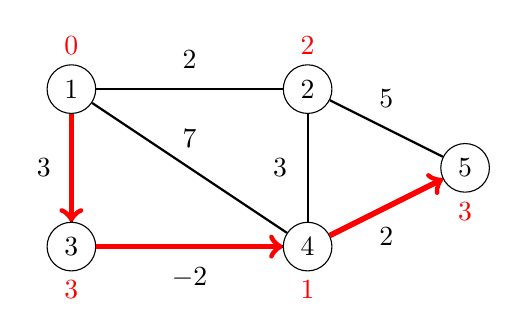
\begin{tikzpicture}
\node[draw, circle] (1) at (1,3) {1};
\node[draw, circle] (2) at (4,3) {2};
\node[draw, circle] (3) at (1,1) {3};
\node[draw, circle] (4) at (4,1) {4};
\node[draw, circle] (5) at (6,2) {5};
\node[color=red] at (1,3+0.55) {$0$};
\node[color=red] at (4,3+0.55) {$2$};
\node[color=red] at (1,1-0.55) {$3$};
\node[color=red] at (4,1-0.55) {$1$};
\node[color=red] at (6,2-0.55) {$3$};
\path[draw,thick,-] (1) -- node[font=\small,label=above:2] {} (2);
\path[draw,thick,-] (1) -- node[font=\small,label=left:3] {} (3);
\path[draw,thick,-] (3) -- node[font=\small,label=below:$-2$] {} (4);
\path[draw,thick,-] (2) -- node[font=\small,label=left:3] {} (4);
\path[draw,thick,-] (2) -- node[font=\small,label=above:5] {} (5);
\path[draw,thick,-] (4) -- node[font=\small,label=below:2] {} (5);
\path[draw,thick,-] (1) -- node[font=\small,label=above:7] {} (4);

\path[draw=red,thick,->,line width=2pt] (1) -- (3);
\path[draw=red,thick,->,line width=2pt] (3) -- (4);
\path[draw=red,thick,->,line width=2pt] (4) -- (5);
\end{tikzpicture}
\end{center}

\subsubsection{Toteutus}

Seuraava Bellman–Fordin algoritmin toteutus
etsii lyhimmät polut solmusta $x$
kaikkiin muihin verkon solmuihin.
Koodi olettaa, että verkko on tallennettuna
vieruslistoina taulukossa
\begin{lstlisting}
vector<pair<int,int>> v[N];
\end{lstlisting}
niin, että parissa on ensin kaaren kohdesolmu
ja sitten kaaren paino.

Algoritmi muodostuu $n-1$ kierroksesta,
joista jokaisella algoritmi käy läpi kaikki
verkon kaaret ja koettaa parantaa etäisyysarvioita.
Algoritmi laskee taulukkoon \texttt{e}
etäisyyden solmusta $x$ kuhunkin verkon solmuun.
Koodissa oleva alkuarvo $10^9$ kuvastaa
ääretöntä.

\begin{lstlisting}
for (int i = 1; i <= n; i++) e[i] = 1e9;
e[x] = 0;
for (int i = 1; i <= n-1; i++) {
    for (int a = 1; a <= n; a++) {
        for (auto b : v[a]) {
            e[b.first] = min(e[b.first],e[a]+b.second);
        }
    }
}
\end{lstlisting}

Algoritmin aikavaativuus on $O(nm)$,
koska se muodostuu $n-1$ kierroksesta ja
käy läpi jokaisen kierroksen aikana kaikki $m$ kaarta.
Jos verkossa ei ole negatiivista sykliä,
kaikki etäisyysarviot ovat lopulliset $n-1$
kierroksen jälkeen, koska jokaisessa lyhimmässä
polussa on enintään $n-1$ kaarta.

Käytännössä kaikki lopulliset etäisyysarviot
saadaan usein laskettua selvästi alle $n-1$ kierroksessa,
joten mahdollinen tehostus algoritmiin on lopettaa heti,
kun mikään etäisyysarvio ei parane kierroksen aikana.

\subsubsection{Negatiivinen sykli}

\index{negatiivinen sykli@negatiivinen sykli}

Bellman–Fordin algoritmin avulla voi myös tarkastaa,
onko verkossa sykliä,
jonka pituus on negatiivinen.
Esimerkiksi verkossa

\begin{center}
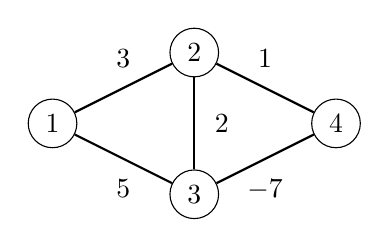
\begin{tikzpicture}[scale=0.9]
\node[draw, circle] (1) at (0,0) {$1$};
\node[draw, circle] (2) at (2,1) {$2$};
\node[draw, circle] (3) at (2,-1) {$3$};
\node[draw, circle] (4) at (4,0) {$4$};

\path[draw,thick,-] (1) -- node[font=\small,label=above:$3$] {} (2);
\path[draw,thick,-] (2) -- node[font=\small,label=above:$1$] {} (4);
\path[draw,thick,-] (1) -- node[font=\small,label=below:$5$] {} (3);
\path[draw,thick,-] (3) -- node[font=\small,label=below:$-7$] {} (4);
\path[draw,thick,-] (2) -- node[font=\small,label=right:$2$] {} (3);
\end{tikzpicture}
\end{center}
\noindent
on negatiivinen sykli $2 \rightarrow 3 \rightarrow 4 \rightarrow 2$,
jonka pituus on $-4$.

Jos verkossa on negatiivinen sykli,
sen kautta kulkevaa polkua voi lyhentää äärettömästi
toistamalla negatiivista sykliä uudestaan ja uudestaan,
minkä vuoksi lyhimmän polun käsite ei ole mielekäs.

Negatiivisen syklin voi tunnistaa
Bellman–Fordin algoritmilla
suorittamalla algoritmia $n$ kierrosta.
Jos viimeinen kierros parantaa jotain
etäisyysarviota, verkossa on negatiivinen sykli.
Huomaa, että algoritmi etsii negatiivista sykliä
koko verkon alueelta alkusolmusta välittämättä.

\subsubsection{SPFA-algoritmi}

\index{SPFA-algoritmi}

\key{SPFA-algoritmi} (''Shortest Path Faster Algorithm'')
on Bellman–Fordin algoritmin muunnelma,
joka on usein alkuperäistä algoritmia tehokkaampi.
Se ei tutki joka kierroksella koko verkkoa läpi
parantaakseen etäisyysarvioita, vaan valitsee
tutkittavat kaaret älykkäämmin.

Algoritmi pitää yllä jonoa solmuista,
joiden kautta saattaa pystyä parantamaan etäisyysarvioita.
Algoritmi lisää jonoon aluksi alkusolmun $x$
ja valitsee aina seuraavan
tutkittavan solmun $a$ jonon alusta.
Aina kun kaari $a \rightarrow b$ parantaa
etäisyysarviota, algoritmi lisää jonoon solmun $b$.

Seuraavassa toteutuksessa jonona on \texttt{queue}-rakenne
\texttt{q}. Lisäksi taulukko \texttt{z} kertoo,
onko solmu valmiina jonossa, jolloin algoritmi ei
lisää solmua jonoon uudestaan.

\begin{lstlisting}
for (int i = 1; i <= n; i++) e[i] = 1e9;
e[x] = 0;
q.push(x);
while (!q.empty()) {
    int a = q.front(); q.pop();
    z[a] = 0;
    for (auto b : v[a]) {
        if (e[a]+b.second < e[b.first]) {
            e[b.first] = e[a]+b.second;
            if (!z[b]) {q.push(b); z[b] = 1;}
        }
    }
}
\end{lstlisting}

SPFA-algoritmin tehokkuus riippuu verkon rakenteesta:
algoritmi on keskimäärin hyvin tehokas, mutta
sen pahimman tapauksen aikavaativuus on edelleen
$O(nm)$ ja on mahdollista
laatia syötteitä, jotka saavat algoritmin yhtä hitaaksi
kuin tavallisen Bellman–Fordin algoritmin.

\section{Dijkstran algoritmi}

\index{Dijkstran algoritmi@Dijkstran algoritmi}

\key{Dijkstran algoritmi} etsii Bellman–Fordin
algoritmin tavoin lyhimmät polut
alkusolmusta kaikkiin muihin solmuihin.
Dijkstran algoritmi on tehokkaampi kuin
Bellman–Fordin algoritmi,
minkä ansiosta se soveltuu suurten
verkkojen käsittelyyn.
Algoritmi vaatii kuitenkin,
ettei verkossa ole negatiivisia kaaria.

Dijkstran algoritmi vastaa
Bellman–Fordin algoritmia siinä,
että se pitää
yllä etäisyysarvioita solmuihin
ja parantaa niitä algoritmin aikana.
Algoritmin tehokkuus perustuu
siihen, että sen riittää käydä läpi
verkon kaaret vain kerran
hyödyntäen tietoa,
ettei verkossa ole negatiivisia kaaria.

\subsubsection{Esimerkki}

Tarkastellaan Dijkstran algoritmin toimintaa
seuraavassa verkossa, kun alkusolmuna
on solmu 1:
\begin{center}
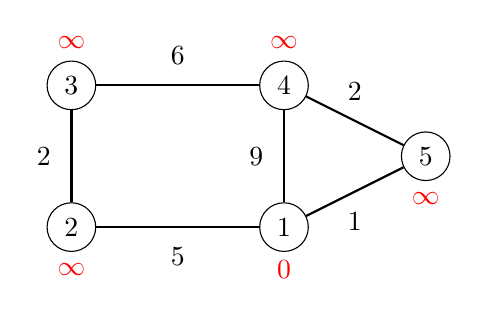
\begin{tikzpicture}[scale=0.9]
\node[draw, circle] (1) at (1,3) {3};
\node[draw, circle] (2) at (4,3) {4};
\node[draw, circle] (3) at (1,1) {2};
\node[draw, circle] (4) at (4,1) {1};
\node[draw, circle] (5) at (6,2) {5};

\node[color=red] at (1,3+0.6) {$\infty$};
\node[color=red] at (4,3+0.6) {$\infty$};
\node[color=red] at (1,1-0.6) {$\infty$};
\node[color=red] at (4,1-0.6) {$0$};
\node[color=red] at (6,2-0.6) {$\infty$};

\path[draw,thick,-] (1) -- node[font=\small,label=above:6] {} (2);
\path[draw,thick,-] (1) -- node[font=\small,label=left:2] {} (3);
\path[draw,thick,-] (3) -- node[font=\small,label=below:5] {} (4);
\path[draw,thick,-] (2) -- node[font=\small,label=left:9] {} (4);
\path[draw,thick,-] (2) -- node[font=\small,label=above:2] {} (5);
\path[draw,thick,-] (4) -- node[font=\small,label=below:1] {} (5);
\end{tikzpicture}
\end{center}
Bellman–Fordin algoritmin tavoin
alkusolmun etäisyysarvio on 0
ja kaikissa muissa solmuissa etäisyysarvio
on aluksi ääretön.

Dijkstran algoritmi
ottaa joka askeleella käsittelyyn
sellaisen solmun,
jota ei ole vielä käsitelty
ja jonka etäisyysarvio on
mahdollisimman pieni.
Alussa tällainen solmu on solmu 1,
jonka etäisyysarvio on 0.

Kun solmu tulee käsittelyyn,
algoritmi käy läpi kaikki
siitä lähtevät kaaret ja
parantaa etäisyysarvioita
niiden avulla:
\begin{center}
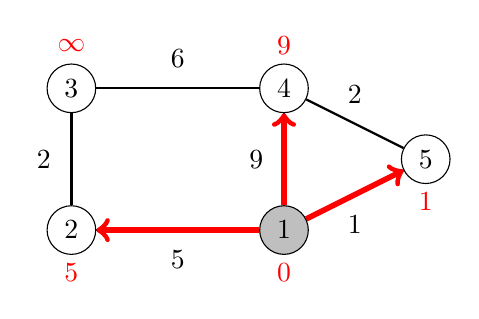
\begin{tikzpicture}[scale=0.9]
\node[draw, circle] (1) at (1,3) {3};
\node[draw, circle] (2) at (4,3) {4};
\node[draw, circle] (3) at (1,1) {2};
\node[draw, circle, fill=lightgray] (4) at (4,1) {1};
\node[draw, circle] (5) at (6,2) {5};

\node[color=red] at (1,3+0.6) {$\infty$};
\node[color=red] at (4,3+0.6) {$9$};
\node[color=red] at (1,1-0.6) {$5$};
\node[color=red] at (4,1-0.6) {$0$};
\node[color=red] at (6,2-0.6) {$1$};

\path[draw,thick,-] (1) -- node[font=\small,label=above:6] {} (2);
\path[draw,thick,-] (1) -- node[font=\small,label=left:2] {} (3);
\path[draw,thick,-] (3) -- node[font=\small,label=below:5] {} (4);
\path[draw,thick,-] (2) -- node[font=\small,label=left:9] {} (4);
\path[draw,thick,-] (2) -- node[font=\small,label=above:2] {} (5);
\path[draw,thick,-] (4) -- node[font=\small,label=below:1] {} (5);

\path[draw=red,thick,->,line width=2pt] (4) -- (2);
\path[draw=red,thick,->,line width=2pt] (4) -- (3);
\path[draw=red,thick,->,line width=2pt] (4) -- (5);
\end{tikzpicture}
\end{center}
Solmun 1 käsittely paransi etäisyysarvioita
solmuihin 2, 4 ja 5,
joiden uudet etäisyydet ovat nyt 5, 9 ja 1.

Seuraavaksi käsittelyyn tulee solmu 5,
jonka etäisyys on 1:
\begin{center}
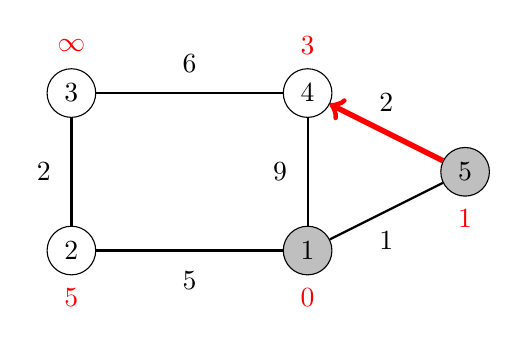
\begin{tikzpicture}
\node[draw, circle] (1) at (1,3) {3};
\node[draw, circle] (2) at (4,3) {4};
\node[draw, circle] (3) at (1,1) {2};
\node[draw, circle, fill=lightgray] (4) at (4,1) {1};
\node[draw, circle, fill=lightgray] (5) at (6,2) {5};

\node[color=red] at (1,3+0.6) {$\infty$};
\node[color=red] at (4,3+0.6) {$3$};
\node[color=red] at (1,1-0.6) {$5$};
\node[color=red] at (4,1-0.6) {$0$};
\node[color=red] at (6,2-0.6) {$1$};

\path[draw,thick,-] (1) -- node[font=\small,label=above:6] {} (2);
\path[draw,thick,-] (1) -- node[font=\small,label=left:2] {} (3);
\path[draw,thick,-] (3) -- node[font=\small,label=below:5] {} (4);
\path[draw,thick,-] (2) -- node[font=\small,label=left:9] {} (4);
\path[draw,thick,-] (2) -- node[font=\small,label=above:2] {} (5);
\path[draw,thick,-] (4) -- node[font=\small,label=below:1] {} (5);

\path[draw=red,thick,->,line width=2pt] (5) -- (2);
\end{tikzpicture}
\end{center}
Tämän jälkeen vuorossa on solmu 4:
\begin{center}
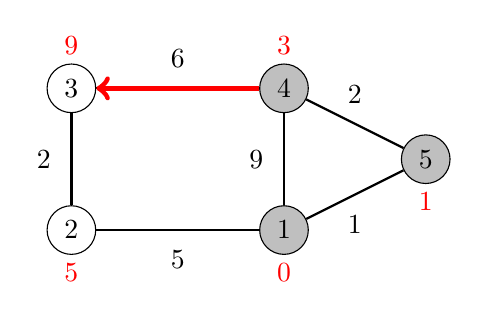
\begin{tikzpicture}[scale=0.9]
\node[draw, circle] (1) at (1,3) {3};
\node[draw, circle, fill=lightgray] (2) at (4,3) {4};
\node[draw, circle] (3) at (1,1) {2};
\node[draw, circle, fill=lightgray] (4) at (4,1) {1};
\node[draw, circle, fill=lightgray] (5) at (6,2) {5};

\node[color=red] at (1,3+0.6) {$9$};
\node[color=red] at (4,3+0.6) {$3$};
\node[color=red] at (1,1-0.6) {$5$};
\node[color=red] at (4,1-0.6) {$0$};
\node[color=red] at (6,2-0.6) {$1$};

\path[draw,thick,-] (1) -- node[font=\small,label=above:6] {} (2);
\path[draw,thick,-] (1) -- node[font=\small,label=left:2] {} (3);
\path[draw,thick,-] (3) -- node[font=\small,label=below:5] {} (4);
\path[draw,thick,-] (2) -- node[font=\small,label=left:9] {} (4);
\path[draw,thick,-] (2) -- node[font=\small,label=above:2] {} (5);
\path[draw,thick,-] (4) -- node[font=\small,label=below:1] {} (5);

\path[draw=red,thick,->,line width=2pt] (2) -- (1);
\end{tikzpicture}
\end{center}

Dijkstran algoritmissa on hienoutena,
että aina kun solmu tulee käsittelyyn,
sen etäisyysarvio on siitä lähtien lopullinen.
Esimerkiksi tässä vaiheessa
etäisyydet 0, 1 ja 3 ovat lopulliset
etäisyydet solmuihin 1, 5 ja 4.

Algoritmi käsittelee vastaavasti
vielä kaksi viimeistä solmua,
minkä jälkeen algoritmin päätteeksi
etäisyydet ovat:

\begin{center}
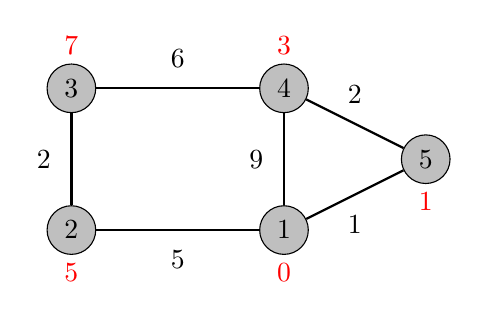
\begin{tikzpicture}[scale=0.9]
\node[draw, circle, fill=lightgray] (1) at (1,3) {3};
\node[draw, circle, fill=lightgray] (2) at (4,3) {4};
\node[draw, circle, fill=lightgray] (3) at (1,1) {2};
\node[draw, circle, fill=lightgray] (4) at (4,1) {1};
\node[draw, circle, fill=lightgray] (5) at (6,2) {5};

\node[color=red] at (1,3+0.6) {$7$};
\node[color=red] at (4,3+0.6) {$3$};
\node[color=red] at (1,1-0.6) {$5$};
\node[color=red] at (4,1-0.6) {$0$};
\node[color=red] at (6,2-0.6) {$1$};

\path[draw,thick,-] (1) -- node[font=\small,label=above:6] {} (2);
\path[draw,thick,-] (1) -- node[font=\small,label=left:2] {} (3);
\path[draw,thick,-] (3) -- node[font=\small,label=below:5] {} (4);
\path[draw,thick,-] (2) -- node[font=\small,label=left:9] {} (4);
\path[draw,thick,-] (2) -- node[font=\small,label=above:2] {} (5);
\path[draw,thick,-] (4) -- node[font=\small,label=below:1] {} (5);
\end{tikzpicture}
\end{center}

\subsubsection{Negatiiviset kaaret}

Dijkstran algoritmin tehokkuus perustuu siihen,
että verkossa ei ole negatiivisia kaaria.
Jos verkossa on negatiivinen kaari,
algoritmi ei välttämättä toimi oikein.
Tarkastellaan esimerkkinä seuraavaa verkkoa:

\begin{center}
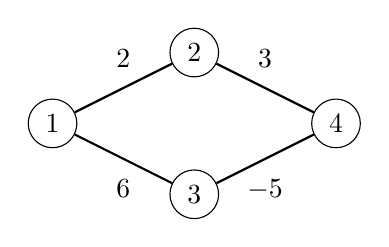
\begin{tikzpicture}[scale=0.9]
\node[draw, circle] (1) at (0,0) {$1$};
\node[draw, circle] (2) at (2,1) {$2$};
\node[draw, circle] (3) at (2,-1) {$3$};
\node[draw, circle] (4) at (4,0) {$4$};

\path[draw,thick,-] (1) -- node[font=\small,label=above:2] {} (2);
\path[draw,thick,-] (2) -- node[font=\small,label=above:3] {} (4);
\path[draw,thick,-] (1) -- node[font=\small,label=below:6] {} (3);
\path[draw,thick,-] (3) -- node[font=\small,label=below:$-5$] {} (4);
\end{tikzpicture}
\end{center}
\noindent
Lyhin polku solmusta 1 solmuun 4 on
$1 \rightarrow 3 \rightarrow 4$,
ja sen pituus on 1.
Dijkstran algoritmi löytää
kuitenkin keveimpiä kaaria seuraten
polun $1 \rightarrow 2 \rightarrow 4$.
Algoritmi ei pysty ottamaan huomioon,
että alemmalla polulla kaaren paino $-5$
kumoaa aiemman suuren kaaren painon $6$.

\subsubsection{Toteutus}

Seuraava Dijkstran algoritmin toteutus laskee
pienimmän etäisyyden solmusta $x$ kaikkiin muihin solmuihin.
Verkko on tallennettu taulukkoon \texttt{v}
vieruslistoina, joissa on pareina kohdesolmu
ja kaaren pituus.

Dijkstran algoritmin tehokas toteutus vaatii,
että verkosta pystyy löytämään
nopeasti vielä käsittelemättömän solmun,
jonka etäisyysarvio on pienin.
Sopiva tietorakenne tähän on prioriteettijono,
jossa solmut ovat järjestyksessä etäisyys\-arvioiden mukaan.
Prioriteettijonon avulla
seuraavaksi käsiteltävän solmun saa selville logaritmisessa ajassa.

Seuraavassa toteutuksessa prioriteettijono sisältää
pareja, joiden ensimmäinen kenttä on etäisyysarvio
ja toinen kenttä on solmun tunniste:
\begin{lstlisting}
priority_queue<pair<int,int>> q;
\end{lstlisting}
Pieni hankaluus on,
että Dijkstran algoritmissa täytyy saada selville
\emph{pienimmän} etäisyysarvion solmu,
kun taas C++:n prioriteettijono antaa oletuksena
\emph{suurimman} alkion.
Helppo ratkaisu on tallentaa etäisyysarviot
\emph{negatiivisina}, jolloin C++:n prioriteettijonoa
voi käyttää suoraan.

Koodi merkitsee taulukkoon \texttt{z},
onko solmu käsitelty,
ja pitää yllä etäisyysarvioita taulukossa \texttt{e}.
Alussa alkusolmun etäisyysarvio on 0
ja jokaisen muun solmun etäisyysarviona
on ääretöntä vastaava $10^9$.

\begin{lstlisting}
for (int i = 1; i <= n; i++) e[i] = 1e9;
e[x] = 0;
q.push({0,x});
while (!q.empty()) {
    int a = q.top().second; q.pop();
    if (z[a]) continue;
    z[a] = 1;
    for (auto b : v[a]) {
        if (e[a]+b.second < e[b]) {
            e[b] = e[a]+b.second;
            q.push({-e[b],b});
        }
    }
}
\end{lstlisting}

Yllä olevan toteutuksen aikavaativuus on $O(n+m \log m)$,
koska algoritmi käy läpi kaikki verkon solmut
ja lisää jokaista kaarta kohden korkeintaan
yhden etäisyysarvion prioriteettijonoon.

\section{Floyd–Warshallin algoritmi}

\index{Floyd–Warshallin algoritmi}

\key{Floyd–Warshallin algoritmi}
on toisenlainen lähestymistapa
lyhimpien polkujen etsintään.
Toisin kuin muut tämän luvun algoritmit,
se  etsii yhdellä kertaa lyhimmät polut kaikkien
verkon solmujen välillä.


Algoritmi ylläpitää kaksiulotteista
taulukkoa etäisyyksistä solmujen
välillä.
Ensin taulukkoon on merkitty
etäisyydet käyttäen vain solmujen
välisiä kaaria.
Tämän jälkeen algoritmi
päivittää etäisyyksiä,
kun verkon solmut saavat yksi kerrallaan
toimia välisolmuina poluilla.

\subsubsection{Esimerkki}

Tarkastellaan Floyd–Warshallin
algoritmin toimintaa seuraavassa verkossa:

\begin{center}
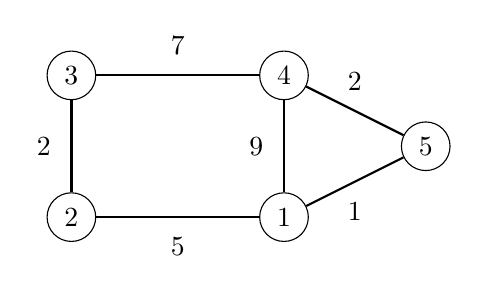
\begin{tikzpicture}[scale=0.9]
\node[draw, circle] (1) at (1,3) {$3$};
\node[draw, circle] (2) at (4,3) {$4$};
\node[draw, circle] (3) at (1,1) {$2$};
\node[draw, circle] (4) at (4,1) {$1$};
\node[draw, circle] (5) at (6,2) {$5$};

\path[draw,thick,-] (1) -- node[font=\small,label=above:7] {} (2);
\path[draw,thick,-] (1) -- node[font=\small,label=left:2] {} (3);
\path[draw,thick,-] (3) -- node[font=\small,label=below:5] {} (4);
\path[draw,thick,-] (2) -- node[font=\small,label=left:9] {} (4);
\path[draw,thick,-] (2) -- node[font=\small,label=above:2] {} (5);
\path[draw,thick,-] (4) -- node[font=\small,label=below:1] {} (5);
\end{tikzpicture}
\end{center}

Algoritmi merkitsee aluksi taulukkoon
etäisyyden 0 jokaisesta solmusta itseensä
sekä etäisyyden $x$, jos solmuparin välillä
on kaari, jonka pituus on $x$.
Muiden solmuparien etäisyys on aluksi ääretön.

Tässä verkossa taulukosta tulee:
\begin{center}
\begin{tabular}{r|rrrrr}
 & 1 & 2 & 3 & 4 & 5 \\
\hline
1 & 0 & 5 & $\infty$ & 9 & 1 \\
2 & 5 & 0 & 2 & $\infty$ & $\infty$ \\
3 & $\infty$ & 2 & 0 & 7 & $\infty$ \\
4 & 9 & $\infty$ & 7 & 0 & 2 \\
5 & 1 & $\infty$ & $\infty$ & 2 & 0 \\
\end{tabular}
\end{center}
\vspace{10pt}
Algoritmin toiminta muodostuu peräkkäisistä kierroksista.
Jokaisella kierroksella valitaan yksi uusi solmu,
joka saa toimia välisolmuna poluilla,
ja algoritmi parantaa taulukon
etäisyyksiä muodostaen polkuja tämän solmun avulla.

Ensimmäisellä kierroksella solmu 1 on välisolmu.
Tämän ansiosta solmujen 2 ja 4 välille muodostuu
polku, jonka pituus on 14,
koska solmu 1 yhdistää ne toisiinsa.
Vastaavasti solmut 2 ja 5 yhdistyvät polulla,
jonka pituus on 6.

\begin{center}
\begin{tabular}{r|rrrrr}
 & 1 & 2 & 3 & 4 & 5 \\
\hline
1 & 0 & 5 & $\infty$ & 9 & 1 \\
2 & 5 & 0 & 2 & \textbf{14} & \textbf{6} \\
3 & $\infty$ & 2 & 0 & 7 & $\infty$ \\
4 & 9 & \textbf{14} & 7 & 0 & 2 \\
5 & 1 & \textbf{6} & $\infty$ & 2 & 0 \\
\end{tabular}
\end{center}
\vspace{10pt}

Toisella kierroksella solmu 2 saa toimia välisolmuna.
Tämä mahdollistaa uudet polut solmuparien 1 ja 3
sekä 3 ja 5 välille:

\begin{center}
\begin{tabular}{r|rrrrr}
 & 1 & 2 & 3 & 4 & 5 \\
\hline
1 & 0 & 5 & \textbf{7} & 9 & 1 \\
2 & 5 & 0 & 2 & 14 & 6 \\
3 & \textbf{7} & 2 & 0 & 7 & \textbf{8} \\
4 & 9 & 14 & 7 & 0 & 2 \\
5 & 1 & 6 & \textbf{8} & 2 & 0 \\
\end{tabular}
\end{center}
\vspace{10pt}

Kolmannella kierroksella solmu 3 saa toimia välisolmuna,
jolloin syntyy uusi polku solmuparin 2 ja 4 välille:

\begin{center}
\begin{tabular}{r|rrrrr}
 & 1 & 2 & 3 & 4 & 5 \\
\hline
1 & 0 & 5 & 7 & 9 & 1 \\
2 & 5 & 0 & 2 & \textbf{9} & 6 \\
3 & 7 & 2 & 0 & 7 & 8 \\
4 & 9 & \textbf{9} & 7 & 0 & 2 \\
5 & 1 & 6 & 8 & 2 & 0 \\
\end{tabular}
\end{center}
\vspace{10pt}


Algoritmin toiminta jatkuu samalla tavalla
niin, että kukin solmu tulee vuorollaan
välisolmuksi.
Algoritmin päätteeksi taulukko sisältää
lyhimmän etäisyyden minkä tahansa
solmuparin välillä:

\begin{center}
\begin{tabular}{r|rrrrr}
 & 1 & 2 & 3 & 4 & 5 \\
\hline
1 & 0 & 5 & 7 & 3 & 1 \\
2 & 5 & 0 & 2 & 9 & 6 \\
3 & 7 & 2 & 0 & 7 & 8 \\
4 & 3 & 9 & 7 & 0 & 2 \\
5 & 1 & 6 & 8 & 2 & 0 \\
\end{tabular}
\end{center}

Esimerkiksi taulukosta selviää, että lyhin polku
solmusta 2 solmuun 4 on pituudeltaan 8.
Tämä vastaa seuraavaa polkua:

\begin{center}
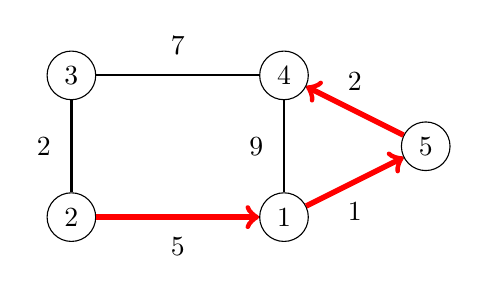
\begin{tikzpicture}[scale=0.9]
\node[draw, circle] (1) at (1,3) {$3$};
\node[draw, circle] (2) at (4,3) {$4$};
\node[draw, circle] (3) at (1,1) {$2$};
\node[draw, circle] (4) at (4,1) {$1$};
\node[draw, circle] (5) at (6,2) {$5$};

\path[draw,thick,-] (1) -- node[font=\small,label=above:7] {} (2);
\path[draw,thick,-] (1) -- node[font=\small,label=left:2] {} (3);
\path[draw,thick,-] (3) -- node[font=\small,label=below:5] {} (4);
\path[draw,thick,-] (2) -- node[font=\small,label=left:9] {} (4);
\path[draw,thick,-] (2) -- node[font=\small,label=above:2] {} (5);
\path[draw,thick,-] (4) -- node[font=\small,label=below:1] {} (5);

\path[draw=red,thick,->,line width=2pt] (3) -- (4);
\path[draw=red,thick,->,line width=2pt] (4) -- (5);
\path[draw=red,thick,->,line width=2pt] (5) -- (2);
\end{tikzpicture}
\end{center}

\subsubsection{Toteutus}

Floyd–Warshallin algoritmin etuna on,
että se on helppoa toteuttaa.
Seuraava toteutus muodostaa etäisyysmatriisin
\texttt{d}, jossa $\texttt{d}[a][b]$
on pienin etäisyys polulla solmusta $a$ solmuun $b$.
Aluksi algoritmi alustaa matriisin \texttt{d}
verkon vierusmatriisin \texttt{v} perusteella
(arvo $10^9$ kuvastaa ääretöntä):

\begin{lstlisting}
for (int i = 1; i <= n; i++) {
    for (int j = 1; j <= n; j++) {
        if (i == j) d[i][j] = 0;
        else if (v[i][j]) d[i][j] = v[i][j];
        else d[i][j] = 1e9;
    }
}
\end{lstlisting}

Tämän jälkeen lyhimmät polut löytyvät seuraavasti:

\begin{lstlisting}
for (int k = 1; k <= n; k++) {
    for (int i = 1; i <= n; i++) {
        for (int j = 1; j <= n; j++) {
            d[i][j] = min(d[i][j], d[i][k]+d[k][j]);
        }
    }
}
\end{lstlisting}

Algoritmin aikavaativuus on
$O(n^3)$, koska siinä on kolme sisäkkäistä
silmukkaa,
jotka käyvät läpi verkon solmut.

Koska Floyd–Warshallin
algoritmin toteutus on yksinkertainen,
algoritmi voi olla hyvä valinta jopa silloin,
kun haettavana on yksittäinen
lyhin polku verkossa.
Tämä on kuitenkin mahdollista vain silloin,
kun verkko on niin pieni,
että kuutiollinen aikavaativuus on riittävä.
